\protect\hyperlink{main-nav}{≡} \protect\hyperlink{close-nav}{×}

\hypertarget{section-2.11-implicit-differentiation-and-related-rates}{%
\section{Section 2.11: Implicit Differentiation and Related
Rates}\label{section-2.11-implicit-differentiation-and-related-rates}}

\hypertarget{implicit-differentiation}{%
\subsection{Implicit Differentiation}\label{implicit-differentiation}}

In our work up until now, the functions we needed to differentiate were
either given explicitly, such as \textbackslash{}( y=x\^{}2+e\^{}x
\textbackslash{}), or it was possible to get an explicit formula for
them, such as solving \textbackslash{}( y\^{}3-3x\^{}2=5
\textbackslash{}) to get \textbackslash{}(
y=\textbackslash{}sqrt{[}3{]}\{5+3x\^{}2\} \textbackslash{}). Sometimes,
however, we will have an equation relating
\textbackslash{}(x\textbackslash{}) and
\textbackslash{}(y\textbackslash{}) which is either difficult or
impossible to solve explicitly for \textbackslash{}(y\textbackslash{}),
such as \textbackslash{}( y+e\^{}y=x\^{}2 \textbackslash{}). In any
case, we can still find \textbackslash{}(y' = f'(x)\textbackslash{}) by
using implicit differentiation.

The key idea behind implicit differentiation is to \textbf{assume that
\textbackslash{}(y\textbackslash{}) is a function of
\textbackslash{}(x\textbackslash{})} even if we cannot explicitly solve
for \textbackslash{}(y\textbackslash{}). This assumption does not
require any work, but we need to be very careful to treat
\textbackslash{}(y\textbackslash{}) as a function when we differentiate
and to use the Chain Rule.

To view this video please enable JavaScript, and consider upgrading to a
web browser that \href{http://videojs.com/html5-video-support/}{supports
HTML5 video}

\hypertarget{example-1}{%
\paragraph{Example 1}\label{example-1}}

Assume that \textbackslash{}(y\textbackslash{}) is a function of
\textbackslash{}(x\textbackslash{}). Calculate

\begin{enumerate}
\tightlist
\item
  \textbackslash{}( \textbackslash{}frac\{d\}\{dx\}\textbackslash{}left(
  y\^{}3 \textbackslash{}right) \textbackslash{})
\item
  \textbackslash{}( \textbackslash{}frac\{d\}\{dx\}\textbackslash{}left(
  x\^{}3y\^{}2 \textbackslash{}right) \textbackslash{})
\item
  \textbackslash{}( \textbackslash{}frac\{d\}\{dx\}\textbackslash{}left(
  \textbackslash{}ln(y) \textbackslash{}right) \textbackslash{})
\end{enumerate}

\begin{enumerate}
\tightlist
\item
  We need the chain rule since y is a function of x: \textbackslash{}{[}
  \textbackslash{}frac\{d\}\{dx\}\textbackslash{}left( y\^{}3
  \textbackslash{}right)=3y\^{}2\textbackslash{}frac\{dy\}\{dx\}\textbackslash{}overset\{\textbackslash{}text\{or\}\}\{=\}3y\^{}2y'
  \textbackslash{}{]}
\item
  We need to use the product rule and the Chain Rule:
  \textbackslash{}{[} \textbackslash{}begin\{align*\}
  \textbackslash{}frac\{d\}\{dx\}\textbackslash{}left( x\^{}3y\^{}2
  \textbackslash{}right)=\&
  x\^{}3\textbackslash{}frac\{d\}\{dx\}\textbackslash{}left( y\^{}2
  \textbackslash{}right)+y\^{}2\textbackslash{}frac\{d\}\{dx\}\textbackslash{}left(
  x\^{}3\textbackslash{}right) \textbackslash{}\textbackslash{} =\&
  x\^{}32y\textbackslash{}frac\{dy\}\{dx\}+y\^{}23x\^{}2
  \textbackslash{}\textbackslash{}
  \textbackslash{}overset\{\textbackslash{}text\{or\}\}\{=\}\&
  2x\^{}3yy'+3y\^{}2x\^{}2 \textbackslash{}end\{align*\}
  \textbackslash{}{]}
\item
  We know \textbackslash{}(
  \textbackslash{}frac\{d\}\{dx\}\textbackslash{}left(
  \textbackslash{}ln(x) \textbackslash{}right)
  =\textbackslash{}frac\{1\}\{x\} \textbackslash{}), so we use that and
  the Chain Rule: \textbackslash{}{[}
  \textbackslash{}frac\{d\}\{dx\}\textbackslash{}left(
  \textbackslash{}ln(y)
  \textbackslash{}right)=\textbackslash{}frac\{1\}\{y\}\textbackslash{}cdot
  y' \textbackslash{}{]}
\end{enumerate}

\hypertarget{implicit-differentiation-1}{%
\paragraph{Implicit Differentiation}\label{implicit-differentiation-1}}

To determine \textbackslash{}(y'\textbackslash{}), differentiate each
side of the defining equation, treating
\textbackslash{}(y\textbackslash{}) as a function of
\textbackslash{}(x\textbackslash{}), and then algebraically solve for
\textbackslash{}(y'\textbackslash{}).

To view this video please enable JavaScript, and consider upgrading to a
web browser that \href{http://videojs.com/html5-video-support/}{supports
HTML5 video}

(The last example in the following video gets rather messy -- don't
worry too much if you can't follow all of the simplifications at the
end.)

To view this video please enable JavaScript, and consider upgrading to a
web browser that \href{http://videojs.com/html5-video-support/}{supports
HTML5 video}

\hypertarget{example-2}{%
\paragraph{Example 2}\label{example-2}}

Find the slope of the tangent line to the circle \textbackslash{}(x\^{}2
+ y\^{}2 = 25\textbackslash{}) at the point (3,4) using implicit
differentiation.

We differentiate each side of the equation \textbackslash{}(x\^{}2 +
y\^{}2 = 25\textbackslash{}) and then solve for
\textbackslash{}(y'\textbackslash{}): \textbackslash{}{[}
\textbackslash{}begin\{align*\}
\textbackslash{}frac\{d\}\{dx\}\textbackslash{}left(x\^{}2+y\^{}2\textbackslash{}right)=\&
\textbackslash{}frac\{d\}\{dx\}(25)\textbackslash{}\textbackslash{}
2x+2yy'=\& 0 \textbackslash{}end\{align*\} \textbackslash{}{]}

Solving for \textbackslash{}(y'\textbackslash{}), we have
\textbackslash{}(
y'=-\textbackslash{}frac\{2x\}\{2y\}=-\textbackslash{}frac\{x\}\{y\}
\textbackslash{}), and, at the point (3,4),
\textbackslash{}{[}y'=-\textbackslash{}frac\{3\}\{4\}.\textbackslash{}{]}

\begin{figure}
\centering
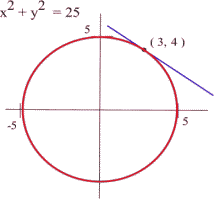
\includegraphics{images/image101.png}
\caption{}
\end{figure}

In the previous example, it would have been easy to explicitly solve for
\textbackslash{}(y\textbackslash{}), and then we could differentiate
\textbackslash{}(y\textbackslash{}) to get
\textbackslash{}(y'\textbackslash{}). Because we could explicitly solve
for \textbackslash{}(y\textbackslash{}), we had a choice of methods for
calculating \textbackslash{}(y'\textbackslash{}). Sometimes, however, we
cannot explicitly solve for \textbackslash{}(y\textbackslash{}), and the
only way of determining \textbackslash{}(y'\textbackslash{}) is to use
implicit differentiation.

To view this video please enable JavaScript, and consider upgrading to a
web browser that \href{http://videojs.com/html5-video-support/}{supports
HTML5 video}

\hypertarget{related-rates}{%
\subsection{Related Rates}\label{related-rates}}

If several variables or quantities are related to each other and some of
the variables are changing at a known rate, then we can use derivatives
to determine how rapidly the other variables must be changing.

Here is a link to the examples used in the videos in this section:
\href{otherfiles/related_rates_math141.pdf}{Related Rates}.

To view this video please enable JavaScript, and consider upgrading to a
web browser that \href{http://videojs.com/html5-video-support/}{supports
HTML5 video}

\hypertarget{example-3}{%
\paragraph{Example 3}\label{example-3}}

Suppose the border of a town is roughly circular, and the radius of that
circle has been increasing at a rate of 0.1 miles each year. Find how
fast the area of the town has been increasing when the radius is 5
miles.

\begin{figure}
\centering
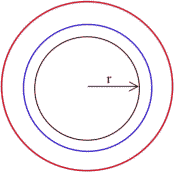
\includegraphics{images/image102.png}
\caption{}
\end{figure}

We could get an \emph{approximate} answer by calculating the area of the
circle when the radius is 5 miles (\textbackslash{}( A =
\textbackslash{}pi r\^{}2 = \textbackslash{}pi (5 \textbackslash{}text\{
miles\})\^{}2 \textbackslash{}approx 78.6 \textbackslash{}text\{
miles\}\^{}2 \textbackslash{}) ) and 1 year later when the radius is 0.1
feet larger than before (\textbackslash{}(A = \textbackslash{}pi r\^{}2
= \textbackslash{}pi (5.1 \textbackslash{}text\{ miles\})\^{}2
\textbackslash{}approx 81.7 \textbackslash{}text\{
miles\}\^{}2\textbackslash{}) ) and then finding \textbackslash{}{[}
\textbackslash{}frac\{\textbackslash{}Delta
\textbackslash{}text\{Area\}\}\{\textbackslash{}Delta
\textbackslash{}text\{time\}\}=\textbackslash{}frac\{81.7
\textbackslash{}text\{ mi\}\^{}2 - 78.6 \textbackslash{}text\{
mi\}\^{}2\}\{1 \textbackslash{}text\{ year\}\} = 3.1
\textbackslash{}text\{
mi\}\^{}2/\textbackslash{}text\{yr\}.\textbackslash{}{]} This
approximate answer represents the average change in area during the 1
year period when the radius increased from 5 miles to 5.1 miles, and
would correspond to the secant slope on the area graph.

To find the exact answer, though, we need derivatives. In this case both
radius and area are functions of time:
\textbackslash{}{[}r(t)=\textbackslash{}text\{ radius at time \} t
\textbackslash{}qquad A(t)=\textbackslash{}text\{ area at time \}
t\textbackslash{}{]}

We know how fast the radius is changing, which is a statement about the
derivative: \textbackslash{}(
\textbackslash{}frac\{dr\}\{dt\}=0.1\textbackslash{}frac\{\textbackslash{}text\{mile\}\}\{\textbackslash{}text\{year\}\}
\textbackslash{}). We also know that \textbackslash{}(r =
5\textbackslash{}) at our moment of interest.

We are looking for how fast the area is increasing, which is
\textbackslash{}( \textbackslash{}frac\{dA\}\{dt\} \textbackslash{}).

Now we need an equation relating our variables, which is the area
equation: \textbackslash{}{[}A=\textbackslash{}pi
r\^{}2.\textbackslash{}{]}

Taking the derivative of both sides of that equation with respect to
\textbackslash{}(t\textbackslash{}), we can use implicit
differentiation: \textbackslash{}{[} \textbackslash{}begin\{align*\}
\textbackslash{}frac\{d\}\{dt\}\textbackslash{}left( A
\textbackslash{}right)=\&
\textbackslash{}frac\{d\}\{dt\}\textbackslash{}left( \textbackslash{}pi
r\^{}2 \textbackslash{}right)\textbackslash{}\textbackslash{}
\textbackslash{}frac\{dA\}\{dt\}=\& \textbackslash{}pi
2r\textbackslash{}frac\{dr\}\{dt\} \textbackslash{}end\{align*\}
\textbackslash{}{]}

Plugging in the values we know for \textbackslash{}(r\textbackslash{})
and \textbackslash{}(\textbackslash{}frac\{dr\}\{dt\}\textbackslash{}),
\textbackslash{}{[} \textbackslash{}frac\{dA\}\{dt\}=\textbackslash{}pi
2(5\textbackslash{}text\{
miles\})\textbackslash{}left(0.1\textbackslash{}frac\{\textbackslash{}text\{miles\}\}\{\textbackslash{}text\{year\}\}\textbackslash{}right)=\textbackslash{}pi\textbackslash{}frac\{\textbackslash{}text\{miles\}\^{}2\}\{\textbackslash{}text\{year\}\}\textbackslash{}{]}

So the area of the town is increasing by approximately 3.14 square miles
per year when the radius is 5 miles.

\hypertarget{related-rates-1}{%
\paragraph{Related Rates}\label{related-rates-1}}

When working with a related rates problem,

\begin{enumerate}
\tightlist
\item
  Draw a picture (if possible).
\item
  Identify the quantities that are changing, and assign them variables.
\item
  Find an equation that relates those quantities.
\item
  Differentiate both sides of that equation with respect to time.
\item
  Plug in any known values for the variables or rates of change.
\item
  Solve for the desired rate.
\end{enumerate}

To view this video please enable JavaScript, and consider upgrading to a
web browser that \href{http://videojs.com/html5-video-support/}{supports
HTML5 video}

\hypertarget{example-4}{%
\paragraph{Example 4}\label{example-4}}

A company has determined the demand curve for their product is
\textbackslash{}( q=\textbackslash{}sqrt\{5000-p\^{}2\}
\textbackslash{}), where \textbackslash{}(p\textbackslash{}) is the
price in dollars, and \textbackslash{}(q\textbackslash{}) is the
quantity in millions. If weather conditions are driving the price up \$2
a week, find the rate at which demand is changing when the price is
\$40.

The quantities changing are \textbackslash{}(p\textbackslash{}) and
\textbackslash{}(q\textbackslash{}), and we assume they are both
functions of time, \textbackslash{}(t\textbackslash{}), in weeks. We
already have an equation relating the quantities, so we can implicitly
differentiate it. \textbackslash{}{[} \textbackslash{}begin\{align*\}
\textbackslash{}frac\{d\}\{dt\}(q)=\&
\textbackslash{}frac\{d\}\{dt\}\textbackslash{}left(5000-p\^{}2\textbackslash{}right)\^{}\{1/2\}
\textbackslash{}\textbackslash{} \textbackslash{}frac\{dq\}\{dt\}=\&
\textbackslash{}frac\{1\}\{2\}\textbackslash{}left(5000-p\^{}2\textbackslash{}right)\^{}\{-1/2\}\textbackslash{}frac\{d\}\{dt\}\textbackslash{}left(5000-p\^{}2\textbackslash{}right)
\textbackslash{}\textbackslash{} \textbackslash{}frac\{dq\}\{dt\}=\&
\textbackslash{}frac\{1\}\{2\}\textbackslash{}left(5000-p\^{}2\textbackslash{}right)\^{}\{-1/2\}\textbackslash{}left(-2p\textbackslash{}frac\{dp\}\{dt\}\textbackslash{}right)
\textbackslash{}end\{align*\} \textbackslash{}{]}

Using the given information, we know the price is increasing by \$2 per
week when the price is \$40, giving \textbackslash{}(
\textbackslash{}frac\{dp\}\{dt\}=2 \textbackslash{}) when
\textbackslash{}(p = 40\textbackslash{}). Plugging in these values,
\textbackslash{}{[} \textbackslash{}frac\{dq\}\{dt\} =
\textbackslash{}frac\{1\}\{2\}\textbackslash{}left(5000-40\^{}2\textbackslash{}right)\^{}\{-1/2\}\textbackslash{}left(-2(40)(2)\textbackslash{}right)
\textbackslash{}approx -1.37 \textbackslash{}{]}

Demand is falling by 1.37 million items per week.

To view this video please enable JavaScript, and consider upgrading to a
web browser that \href{http://videojs.com/html5-video-support/}{supports
HTML5 video}

To view this video please enable JavaScript, and consider upgrading to a
web browser that \href{http://videojs.com/html5-video-support/}{supports
HTML5 video}

\begin{longtable}[]{@{}ll@{}}
\toprule
\endhead
\href{section2-10.php}{← Previous Section} &
\href{../chapter3/section3-1.php}{Next Section →}\tabularnewline
\bottomrule
\end{longtable}
